\documentclass[10pt,a4paper]{article}
\usepackage[utf8]{inputenc}
\usepackage{amsmath}
\usepackage{amsfonts}
\usepackage{amssymb}
\usepackage{ngerman}
\usepackage[pdftex]{graphicx}
\usepackage{float}
\DeclareGraphicsExtensions{.pdf,.png,.eps,.jpg}
\usepackage{gensymb}
\usepackage[T1]{fontenc}


\author{Gruppe 2 - Felix Friese, Aljoscha Schmidt,\\Stephan Wenninger, Lars Oetermann}
\title{Space Gladiator}
\begin{document}
\maketitle
\section{Synopsis}
In a Space-Arena 2-8 players fight each other while moving with constant speed in Pod-Racer-like vehicles to make the game fast and rich in action. The goal is to score the most points in limited time by destorying enemies with laser-projectiles and different items which lead to an unpredictable gameplay. A destroyed player respawns with a new vehicle and can continue playing and scoring points. In contrast to reality damaged vihicles move with increased speed.\\
\\
In einer Space-Arena kämpfen 2-8 Spieler gegeneinander, wobei sie sich in Fahrzeugen (Pod-Racer) mit konstanter Geschwindigkeit bewegen, wodurch das Spiel schnell und actiongeladen wird. Ziel ist es in begrenzter Zeit, die meisten Punkte durch das Zerstören von Gegnern zu sammeln, in dem diese mit Laser-Projeketilen beschossen werden oder verschiedene Items verwendet werden, die eine gewissen Unberechenbarkeit hinzufügen. Zerstörte Spieler respawnen mit einem neuen Fahrzeug um nicht direkt auszuscheiden und weiterhin Punkte sammeln zu können. Im Gegensatz zur Realität bewegen sich beschädigte Fahrzeuge mit erhöhter Geschwindigkeit.

\section{Story}
Starsystem Heleris. Year 4365.\\
The interplanetary dictator has ruled that for the entertainment of the citizens and the demonstration of his power, slaves from each planet are sent to fight in an arena for survival. Only the final winner will survive and receive his freedom.\\
However Aron McRode would rather have stayed and worked on the field on planet Isiris which was a home to him and his family. It was hard work but at least they did not suffer and it was safe. At the end they did not let him make any decision but between winning or dying.\\
Can Aron win all his matches to take part in the grand final or will we see an unexpected twist of events during the fight for freedom?

\section{Gameplay}
\subsection{Interaction Pattern}
Single-Player vs Game or Players vs Players / Multilateral Competition \\
\subsection{Objective}
\begin{enumerate}
  \item Chase and kill other Players
  \item Forbidden Act: Fall out of the map
\end{enumerate}
\subsubsection{Procedures}
Move on grid (only multiples of 90 degrees), shoot freely (maybe place walls to create convoys)\\
Input-Devices: Mouse and Keyboard, Gamepad \\
Resource: Health \\
Maybe: Power-Ups (collectable Items that are dropped by defeated enemies and that modify game mechanics) e.g. a reversed gun: projectiles are spawned on the map, and
that gun attracts that projectile, so that the player has to position himself so that the enemy gets hit.\\
(maybe special terrain)
\subsection{Rewards}
special items, points

\section{Visualization}


\begin{figure}[H]
  \centering
  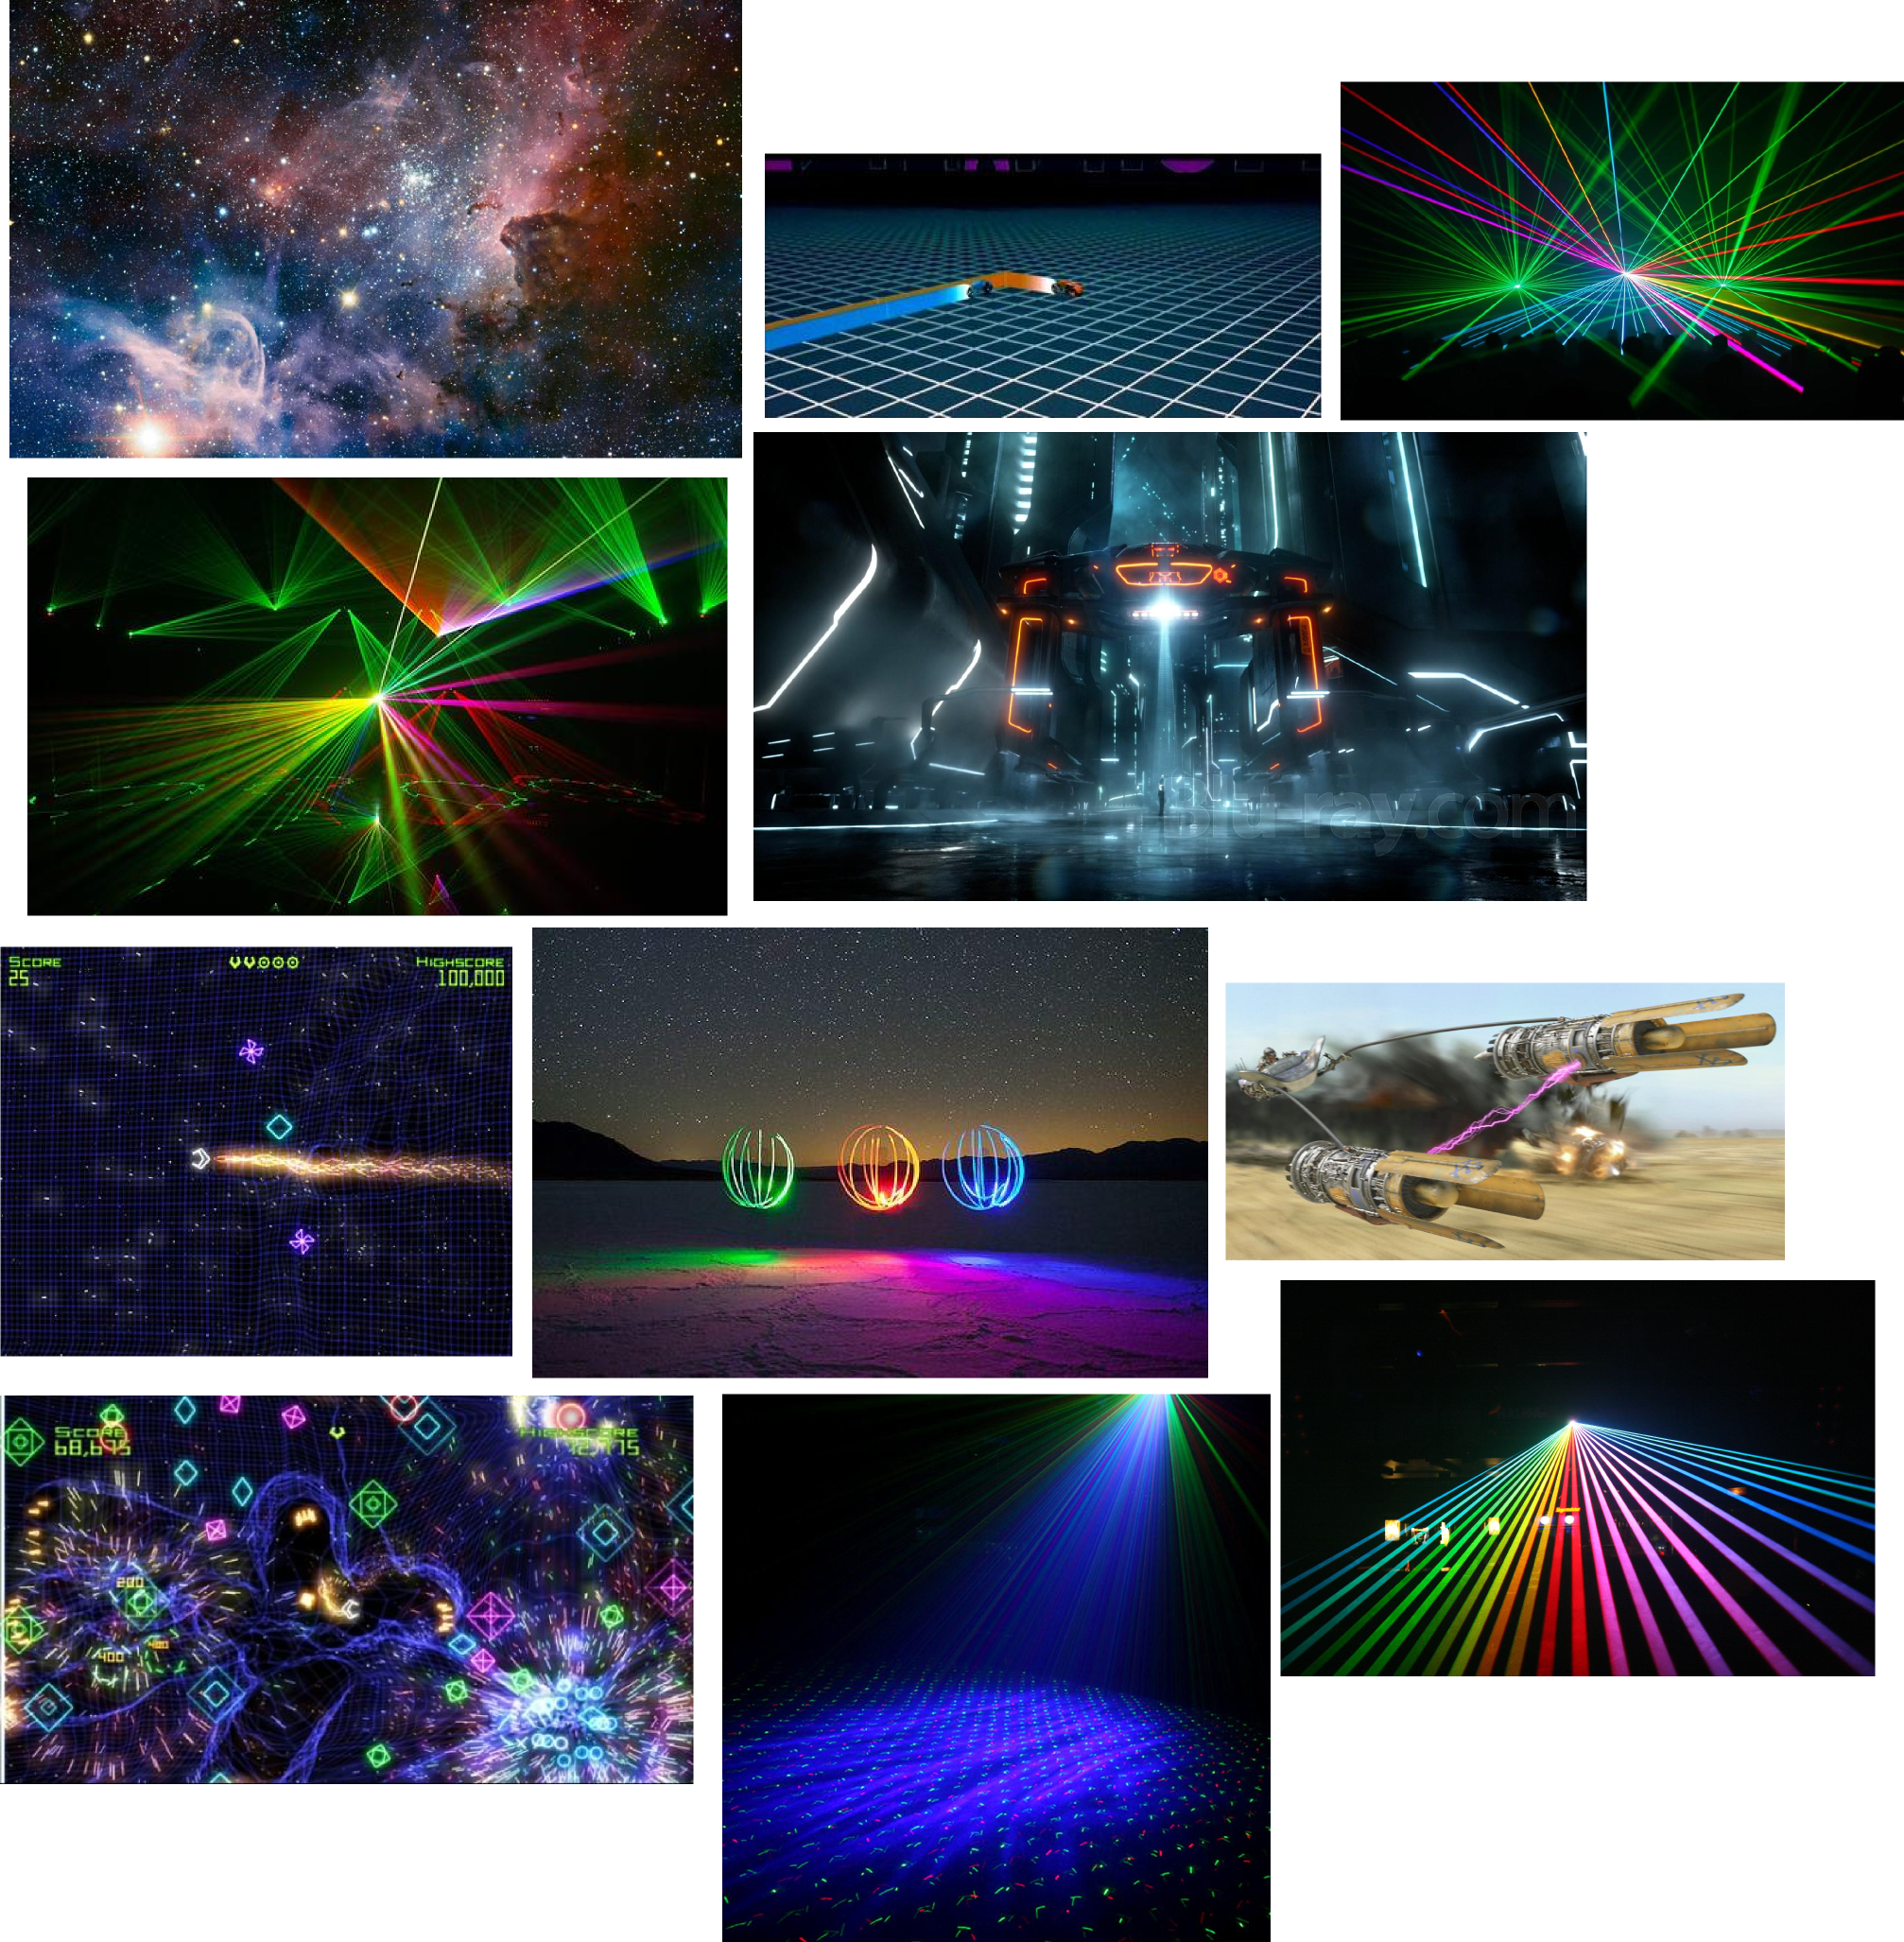
\includegraphics[width=0.7\textwidth]{collage.png}
  \caption{Collage of the Look and Feel of the game. Inspiration comes from Tron, Star Wars, Geometry Wars and generally Laser and Neon styles.}
  \label{fig:figure1}
\end{figure}

\begin{figure}[H]
  \centering
  \includegraphics[width=0.3\textwidth]{colorpalette2.png}
  \caption{We want to use mainly rainbow Colors on dark backgrounds to provide a futuristic spacy look. Glowing effects will provide a neon look.}
  \label{fig:figure2}
\end{figure}

\begin{figure}[H]
  \centering
  \includegraphics[width=0.3\textwidth]{sketch.png}
  \label{fig:figure3}
  \caption{Rough sketch. Missing bloom/particle effects, ongoing shooting and multiple players.}
\end{figure}

\begin{figure}[H]
  \centering
  \includegraphics[width=0.5\textwidth]{itemslook.png}
  \caption{Items will be flat icons spinning in neon cages. The Vehicles will be an hommage to podracer from Star Wars but placed in a neon/laser setting.}
  \label{fig:figure4}
\end{figure}

\section{Technical challenges}

For developing a multiplayer game that features enemies controlled by
the computer, it is a crucial and complex task to design a suitable
artificial intelligence. There are multiple challenges for implementing
an AI that provide challenging, yet not invincible computer-controlled
opponents for our game. First, the paths that are taken by the AI need
to be strategic, at least to some extent, rather than simply random or
easily predictable (e.g. moving straight toward opponents or fleeing
from them). To achieve this, an applicable heuristic needs to be
created. Additionally, algorithms for simulating a field of view, target
selection, aiming, and usage of items and abilities are required to
create opponents that behave similar to human players or at the minimum
offer appropriate competition.\\
\\
Other general challenges for the game include, but are not limited to
the graphical effects (e.g. particle effects), character animations,
implementation of items and abilities, possibly online- or networking
features, as well as balancing the mechanics to establish a
well-adjusted and enjoyable multiplayer gameplay. Especially the latter
is an essential part, and might require some time to realize satisfactorily.

\end{document}